\documentclass[border=15pt, multi, tikz]{standalone}
\usepackage{import}
\subimport{../../layers/}{init}
\usetikzlibrary{positioning}
\usetikzlibrary{3d} %for including external image 
\usetikzlibrary {calc,arrows.meta,positioning}
%\documentclass{article}
%\usepackage{tikz}

%\setmainfont{Helvetica};

\def\ConvColor{rgb:green,5;yellow,7}
\def\DoubleConv{rgb:magenta,5;black,7}
\def\DenseBlockColor{rgb:violet,5;blue,2}
\def\ConvReluColor{rgb:yellow,5;red,5;white,5}
\def\PoolColor{rgb:blue,1;green,1;black,0.3}
\def\DcnvColor{rgb:blue,5;green,2.5;white,5}
\def\SoftmaxColor{rgb:red,5;brown,1}
\def\SumColor{rgb:blue,5;green,15}
\def\ConvTransColor{rgb:yellow,5;red,5;white,5}

%\def\ConvColor{rgb:yellow,5;red,2.5;white,5}
%\def\ConvReluColor{rgb:yellow,5;red,5;white,5}
%\def\PoolColor{rgb:red,1;black,0.3}
\def\UnpoolColor{rgb:blue,5;green,3.5;black,0.3}
\def\SigmoidColor{rgb:blue,5;yellow,3.5;black,0.3}

\def\BlueColor{rgb: blue, 5} 
\def\RedColor{rgb: red, 10} 

\def\FcColor{rgb:blue,5;red,2.5;white,5}
\def\FcReluColor{rgb:blue,5;red,5;white,4}
%\def\SoftmaxColor{rgb:yellow,5;red,2.5;white,5}
\def\ConcatColor{rgb:blue,4;red,1;green,1;black,3}
\newcommand{\copymidarrow}{\tikz \draw[-Stealth,line width =0.8mm,draw={rgb:blue,4;red,1;green,1;black,3}] (-0.3,0) -- ++(0.3,0);}
\def\aPoolColor{rgb: red,3; orange, 3; blue, 3}   

\begin{document}
\begin{tikzpicture}
\tikzstyle{connection}=[ultra thick,every node/.style={sloped,allow upside down},draw=\edgecolor,opacity=0.7]
\tikzstyle{arc connection}=[connection, to path={
  (\tikztostart) to[out=0, in=180] (\tikztotarget) \tikztonodes
}]


\tikzstyle{connection}=[ultra thick,every node/.style={sloped,allow upside down},draw=\edgecolor,opacity=0.7]
\tikzstyle{copyconnection}=[ultra thick,every node/.style={sloped,allow upside down},draw={rgb:blue,4;red,1;green,1;black,3},opacity=0.7]
%%%%%%%%%%%%%%%%%%%%%%%%%%%%%%%%%%%%%%%%%%%%%%%%%%%%%%%%%%%%%%%%%%%%%%%%%%%%%%%%%%%%%%%%
%% Draw Layer Blocks
%%%%%%%%%%%%%%%%%%%%%%%%%%%%%%%%%%%%%%%%%%%%%%%%%%%%%%%%%%%%%%%%%%%%%%%%%%%%%%%%%%%%%%%%
\node[canvas is zy plane at x=0] (temp) at (0,0,0) {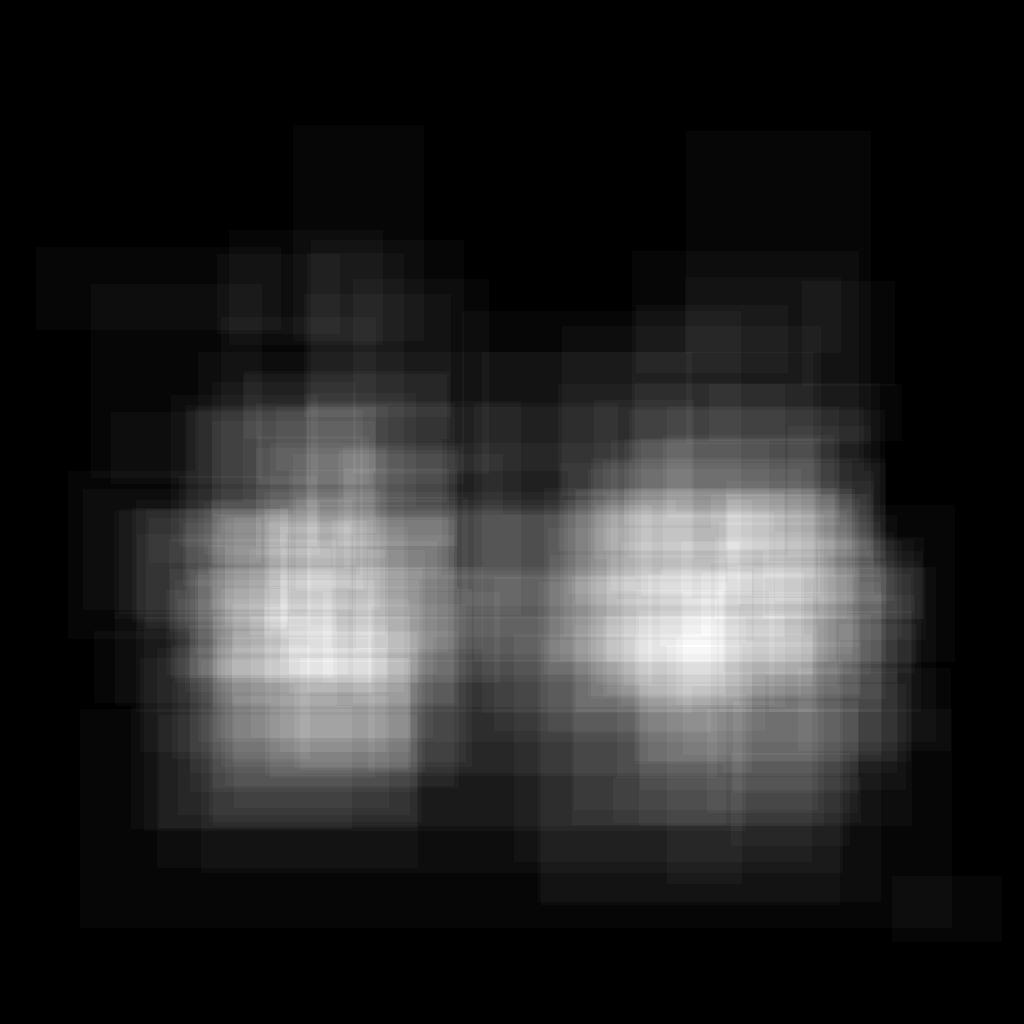
\includegraphics[width=9cm,height=9cm]{mask_0.jpg}};
\pic[shift={(9,0,0)}] at (temp) {Box={name=downsamplemask,%
        caption=,zlabel=,fill=\aPoolColor,font=\huge,
        height=35,width={2},depth=35}};
\node[text width=20cm, align=center,font=\Huge\sffamily, shift={(0,-2.5,0)}] at (downsamplemask-south) {Down Sample to (HxW)};



\pic[shift={(13,0)}] at (temp) {Ball={name=dot1,fill=\BlueColor,opacity=0,radius=3,logo=\Huge$\cdot$}};  


\pic[shift={(16,0,0)}] at (temp) {Box={name=f1,%
        caption=(HxWxC),zlabel=,fill=\RedColor,font=\huge,
        height=35,width={0.2},depth=35}};
\pic[shift={(.3,0,0)}] at (f1-west) {Box={name=f2,%
        caption=,zlabel=,fill=\RedColor,font=\Huge,
        height=35,width={0.2},depth=35}};
\pic[shift={(.6,0,0)}] at (f1-west) {Box={name=f3,%
        caption=,zlabel=,fill=\RedColor,
        height=35,width={0.2},depth=35}};
\pic[shift={(.9,0,0)}] at (f1-west) {Box={name=f4,%
        caption=,zlabel=,fill=\RedColor,
        height=35,width={0.2},depth=35}};
\node[text width=20cm, align=center,font=\Huge\sffamily, shift={(0,-3,0)}] at (f2-south) {Feature Map};
        
        
%\draw (f4-east)++(5,0,0) -- (m1-east)++(1,0,0) [->,line width=0.5mm, color=\edgecolor];
        
%%%%%%%%%%%%%%%%%%     uper box      %%%%%%%%%%%%%%%%%%%%%%%%%

\pic[shift={(20,0,0)}] at (f4-east) {Box={name=m1,%
        caption=(HxWxC),zlabel=,fill=\BlueColor,font=\huge,
        height=35,width={0.2},depth=35}};
\pic[shift={(.3,0,0)}] at (m1-west) {Box={name=m2,%
        caption=,zlabel=,fill=\BlueColor,
        height=35,width={0.2},depth=35}};
\pic[shift={(.6,0,0)}] at (m1-west) {Box={name=m3,%
        caption=,zlabel=,fill=\BlueColor,
        height=35,width={0.2},depth=35}};
\pic[shift={(.9,0,0)}] at (m1-west) {Box={name=m4,%
        caption=,zlabel=,fill=\BlueColor,font=\Huge,
        height=35,width={0.2},depth=35}};
\node[text width=20cm, align=center,font=\Huge\sffamily, shift={(0,-3,0)}] at (m2-south) {Masked Feature Map};

 
% \pic[shift={(5,0)}] at (temp) {Ball={name=dot1,fill=\BlueColor,opacity=0,radius=3,logo=\Huge$\cdot$}};       
\draw (f4-east)++(5,0,0) --++(10,0,0) [->,line width=0.7mm, color=\edgecolor];
\draw (temp)++(2.5,0,0) --++(4.5,0,0) [->,line width=0.7mm, color=\edgecolor];

\pic[shift={(-5,0,0)}] at (temp) {Box={name=block1,caption=(a),%
        fill=\PoolColor,opacity=0,height=68,width=230,depth=0,font=\Huge,}};


%%%%%%%%%%%%%%%%% upper box ends here with connections %%%%%%%%%%%%%%%
\def\aPoolColor{rgb: red,3; orange, 3; blue, 3}        
\def\batchColor{rgb: blue,5} 
\def\reluColor{rgb: red,3; orange, 3; yellow, 3}       
 
 
 % top section        
\pic[shift={(0,-17,0)}] at (temp) {Box={name=GMP1,%
        caption=GMP,zlabel=,fill=\PoolColor,font=\Huge,
        height=35,width={10},depth=35}};
\pic[shift={(5,0,0)}] at (GMP1-east) {Box={name=GMP1a,%
        caption=Conv 1x1,zlabel=,fill=\ConvColor,font=\Huge,
        height=15,width={20},depth=15}};
%\pic[shift={(2,0,0)}] at (GMP1a-east) {Box={name=GMP1b,%
 %       caption=Batch Norm,zlabel=,fill=\batchColor,font=\Huge,
%        height=15,width={20},depth=15}};
\pic[shift={(2,0,0)}] at (GMP1a-east) {Box={name=GMP1c,%
        caption=Leaky ReLU,zlabel=,fill=\reluColor,font=\Huge,
        height=15,width={20},depth=15}};
\node[text width=20cm, align=center,font=\Huge\sffamily, shift={(5,0,0)}] at (GMP1c-south) {1x1xC};
   
    
\pic[shift={(0,-6,0)}] at (GMP1-southwest) {Box={name=GAP1,%
        caption=GAP,zlabel=,fill=\aPoolColor,font=\Huge,
        height=35,width={10},depth=35}};
\pic[shift={(5,0,0)}] at (GAP1-east) {Box={name=GAP1a,%
        caption=Conv 1x1,zlabel=,fill=\ConvColor,font=\Huge,
        height=15,width={20},depth=15}};
%\pic[shift={(2,0,0)}] at (GAP1a-east) {Box={name=GAP1b,%
%        caption=Batch Norm,zlabel=,fill=\batchColor,font=\Huge,
%        height=15,width={20},depth=15}};
\pic[shift={(2,0,0)}] at (GAP1a-east) {Box={name=GAP1c,%
        caption=Leaky ReLU,zlabel=,fill=\reluColor,font=\Huge,
        height=15,width={20},depth=15}};
 \node[text width=20cm, align=center,font=\Huge\sffamily, shift={(5,0,0)}] at (GAP1c-south) {1x1xC};
\pic[shift={(-3,-5,0)}] at (GMP1-west) {Box={name=toprow,%
        caption=CLR Block,zlabel=,fill=\BlueColor,opacity=0.1,font=\Huge,
        height=105,width={140},depth=40}};
        
        

        
        
 % bottom section        
\pic[shift={(0,-10,0)}] at (GAP1-southwest) {Box={name=GMP2,%
        caption=GMP,zlabel=,fill=\PoolColor,font=\Huge,
        height=35,width={10},depth=35}};
\pic[shift={(5,0,0)}] at (GMP2-east) {Box={name=GMP2a,%
        caption=Conv 1x1,zlabel=,fill=\ConvColor,font=\Huge,
        height=15,width={20},depth=15}};
%\pic[shift={(2,0,0)}] at (GMP2a-east) {Box={name=GMP2b,%
%        caption=Batch Norm,zlabel=,fill=\batchColor,font=\Huge,
%        height=15,width={20},depth=15}};
\pic[shift={(2,0,0)}] at (GMP2a-east) {Box={name=GMP2c,%
        caption=Leaky ReLU,zlabel=,fill=\reluColor,font=\Huge,
        height=15,width={20},depth=15}};
\node[text width=20cm, align=center,font=\Huge\sffamily, shift={(5,0,0)}] at (GMP2c-south) {1x1xC};

\pic[shift={(0,-6,0)}] at (GMP2-southwest) {Box={name=GAP2,%
        caption=GAP,zlabel=,fill=\aPoolColor,font=\Huge,
        height=35,width={10},depth=35}};
\pic[shift={(5,0,0)}] at (GAP2-east) {Box={name=GAP2a,%
        caption=Conv 1x1,zlabel=,fill=\ConvColor,font=\Huge,
        height=15,width={20},depth=15}};
%\pic[shift={(2,0,0)}] at (GAP2a-east) {Box={name=GAP2b,%
%        caption=Batch Norm,zlabel=,fill=\batchColor,font=\Huge,
%        height=15,width={20},depth=15}};
\pic[shift={(2,0,0)}] at (GAP2a-east) {Box={name=GAP2c,%
        caption=Leaky ReLU,zlabel=,fill=\reluColor,font=\Huge,
        height=15,width={20},depth=15}};
        
\node[text width=20cm, align=center,font=\Huge\sffamily, shift={(5,0,0)}] at (GAP2c-south) {1x1xC};
        
\pic[shift={(-3,-5,0)}] at (GMP2-west) {Box={name=bottomrow,%
        caption=CLR Block,zlabel=,fill=\BlueColor,opacity=0.1,font=\Huge,
        height=105,width={140},depth=40}};
        
        
\pic[shift={(-15,-5,0)}] at (GMP1-west) {Box={name=tf,%
        caption=(HxWxC),zlabel=,fill=\BlueColor,font=\huge,
        height=35,width={0.2},depth=35}};
\pic[shift={(.3,0,0)}] at (tf-west) {Box={name=tf1,%
        caption=,zlabel=,fill=\BlueColor,
        height=35,width={0.2},depth=35}};
\pic[shift={(.6,0,0)}] at (tf-west) {Box={name=tf2,%
        caption=,zlabel=,fill=\BlueColor,
        height=35,width={0.2},depth=35}};
\pic[shift={(.9,0,0)}] at (tf-west) {Box={name=tf3,%
        caption=,zlabel=,fill=\BlueColor,font=\Huge,
        height=35,width={0.2},depth=35}};
\node[text width=20cm, align=center,font=\Huge\sffamily, shift={(0.5,-3,0)}] at (tf1-south) {Masked Feature Map};
        
        
\pic[shift={(-15,-5,0)}] at (GMP2-west) {Box={name=bm,%
        caption=(HxWxC),zlabel=,fill=\RedColor,font=\huge,
        height=35,width={0.2},depth=35}};
\pic[shift={(.3,0,0)}] at (bm-west) {Box={name=bm1,%
        caption=,zlabel=,fill=\RedColor,
        height=35,width={0.2},depth=35}};
\pic[shift={(.6,0,0)}] at (bm-west) {Box={name=bm2,%
        caption=,zlabel=,fill=\RedColor,
        height=35,width={0.2},depth=35}};
\pic[shift={(.9,0,0)}] at (bm-west) {Box={name=bm3,%
        caption=,zlabel=,fill=\RedColor,font=\Huge,
        height=35,width={0.2},depth=35}};
 %  box2     
\pic[shift={(-18,-17,0)}] at (GMP1-west) {Box={name=block2,%
        caption=(b),zlabel=,fill=\BlueColor,font=\Huge,opacity=0,
        height=248,width={380},depth=0}};
        
\node[text width=20cm, align=center,font=\Huge\sffamily, shift={(0,-3,0)}] at (bm1-south) {Feature Map};
        
        
        
        
        
        
 % forward section 
 \pic[shift={(8,-10,0)}] at (toprow-east) {Box={name=forwardconv,%
        caption=Conv 1x1,zlabel=,fill=\ConvColor,font=\Huge,
        height=15,width={20},depth=15}};
% \pic[shift={(2,0,0)}] at (forwardconv-east) {Box={name=forwardbatch,%
%        caption=Batch Norm,zlabel=,fill=\batchColor,font=\Huge,
%        height=15,width={20},depth=15}};
 \pic[shift={(2,0,0)}] at (forwardconv-east) {Box={name=forwardsigmoid,%
        caption=Sigmoid,zlabel=,fill=\SigmoidColor,font=\Huge,
        height=15,width={20},depth=15}};
        
 
 \pic[shift={(-1,0,0)}] at (forwardconv-west) {Box={name=forward,%
        caption=CS Block,zlabel=,fill=\BlueColor,opacity=0.1,font=\Huge,
        height=30,width={67},depth=20}};
        
\pic[shift={(8,0,0)}] at (forwardsigmoid-east) {Box={name=output,font=\Huge\sffamily\bfseries, caption={1x1xC}, ylabel=,fill=\ConvColor,height=2,width=2,depth=100}};
\node[text width=20cm, align=center,font=\Huge\sffamily\bfseries, shift={(-3,-6.5,0)}] at (output-south) {Channel Weighting Vector};


\pic[shift={(-4,0,0)}] at (forwardconv-west) {Ball={name=add1,fill={rgb:white, 5},radius=4,logo=$+$}}; 


\draw(tf3-east)[->,line width =0.5mm,color=\edgecolor]--++(5,0,0)--++(0,5,0)--(GMP1-west);
\draw(GMP1-east)[->,line width =0.5mm,color=\edgecolor]--(GMP1a-west);
\draw(GMP1a-east)[->,line width =0.5mm,color=\edgecolor]--(GMP1c-west);
%\draw(GMP1b-east)[->,line width =0.5mm,color=\edgecolor]--(GMP1c-west);
\draw(GMP1c-east)[->,line width =0.5mm,color=\edgecolor]--++(7.4,0,0)--(add1-north);

\draw(tf3-east)[->,line width =0.5mm,color=\edgecolor]--++(5,0,0)--++(0,-4.5,0)--(GAP1-west);
\draw(GAP1-east)[->,line width =0.5mm,color=\edgecolor]--(GAP1a-west);
\draw(GAP1a-east)[->,line width =0.5mm,color=\edgecolor]--(GAP1c-west);
%\draw(GAP1b-east)[->,line width =0.5mm,color=\edgecolor]--(GAP1c-west);
\draw(GAP1c-east)[->,line width =0.5mm,color=\edgecolor]--++(7.4,0,0)--(add1-north);


\draw(bm3-east)[->,line width =0.5mm,color=\edgecolor]--++(5,0,0)--++(0,5,0)--(GMP2-west);
\draw(GMP2-east)[->,line width =0.5mm,color=\edgecolor]--(GMP2a-west);
\draw(GMP2a-east)[->,line width =0.5mm,color=\edgecolor]--(GMP2c-west);
%\draw(GMP2b-east)[->,line width =0.5mm,color=\edgecolor]--(GMP2c-west);
\draw(GMP2c-east)[->,line width =0.5mm,color=\edgecolor]--++(7.4,0,0)--(add1-south);

\draw(bm3-east)[->,line width =0.5mm,color=\edgecolor]--++(5,0,0)--++(0,-4.5,0)--(GAP2-west);
\draw(GAP2-east)[->,line width =0.5mm,color=\edgecolor]--(GAP2a-west);
\draw(GAP2a-east)[->,line width =0.5mm,color=\edgecolor]--(GAP2c-west);
%\draw(GAP2b-east)[->,line width =0.5mm,color=\edgecolor]--(GAP2c-west);
\draw(GAP2c-east)[->,line width =0.5mm,color=\edgecolor]--++(7.4,0,0)--(add1-south);
\draw(add1-east)[->,line width =0.5mm,color=\edgecolor]--(forwardconv-west);
%\draw(forwardconv-east)[->,line width =0.5mm,color=\edgecolor]--(forwardbatch-west);
\draw(forwardconv-east)[->,line width =0.5mm,color=\edgecolor]--(forwardsigmoid-west);
\draw(forwardsigmoid-east)[->,line width =0.5mm,color=\edgecolor]--(output-west);





% section c 

\pic[shift={(-5,-15,0)}] at (GAP2-south) {Box={name=lf,%
        caption=(HxWxC),zlabel=,fill=\BlueColor,font=\huge,
        height=35,width={0.2},depth=35}};
\pic[shift={(.3,0,0)}] at (lf-west) {Box={name=lf1,%
        caption=,zlabel=,fill=\BlueColor,
        height=35,width={0.2},depth=35}};
\pic[shift={(.6,0,0)}] at (lf-west) {Box={name=lf2,%
        caption=,zlabel=,fill=\BlueColor,
        height=35,width={0.2},depth=35}};
\pic[shift={(.9,0,0)}] at (lf-west) {Box={name=lf3,%
        caption=,fill=\BlueColor,font=\Large,
        height=35,width={0.2},depth=35}};
\node[text width=20cm, align=center,font=\Huge\sffamily, shift={(0,-3,0)}] at (lf1-south) {Masked Feature Map};
        

\pic[shift={(10,0,0)}] at (lf3-east) {Box={name=lfconv,%
        caption=Channel Weighting Vector,zlabel=,fill=\ConvColor,font=\Huge,
        height=2,width={50},depth=2}};
\pic[shift={(5,0,0)}] at (lf3-east) {Ball={name=dot2,fill={rgb:white, 5},radius=3,logo=$\cdot$, font=\Huge}};
        
\pic[shift={(-5,-27,0)}] at (GAP2-south) {Box={name=lm,%
        caption=(HxWxC),zlabel=,fill=\RedColor,font=\huge,
        height=35,width={0.2},depth=35}};
\pic[shift={(.3,0,0)}] at (lm-west) {Box={name=lm1,%
        caption=,zlabel=,fill=\RedColor,font=\huge,
        height=35,width={0.2},depth=35}};
\pic[shift={(.6,0,0)}] at (lm-west) {Box={name=lm2,%
        caption=,zlabel=,fill=\RedColor,
        height=35,width={0.2},depth=35}};
\pic[shift={(.9,0,0)}] at (lm-west) {Box={name=lm3,%
        caption=,zlabel=,fill=\RedColor,font=\huge,
        height=35,width={0.2},depth=35}};
\node[text width=20cm, align=center,font=\Huge\sffamily, shift={(0,-3,0)}] at (lm1-south) {Feature Map};

\pic[shift={(10,0,0)}] at (lm3-east) {Box={name=mfconv,%
        caption=1 - Channel Weighting Vector,zlabel=,fill=\ConvColor,font=\Huge,
        height=2,width={50},depth=2}};
        
\pic[shift={(5,0,0)}] at (lm3-east) {Ball={name=dot3,fill={rgb:white, 5},radius=3,logo=$\cdot$, font=\Huge}};
        
\pic[shift={(7.5,-5,0)}] at (lfconv-east) {Ball={name=cat1,fill={rgb:white, 5},radius=4,logo=$+$}}; 

\pic[shift={(5,0,0)}] at (cat1-east) {Box={name=sectcbatch,%
        caption=,zlabel=,fill=\batchColor,font=\Huge,
        height=35,width={7.5},depth=35}};
\node[text width=20cm, align=center,font=\Huge\sffamily, shift={(0,-2.5,0)}] at (sectcbatch-south) {Batch Norm};
        
\pic[shift={(20,-5,0)}] at (lfconv-east) {Box={name=lfc,%
        caption=(HxWxC),zlabel=,fill={rgb:magenta, 5},font=\huge,
        height=35,width={0.2},depth=35}};
\pic[shift={(.3,0,0)}] at (lfc-west) {Box={name=lfc1,%
        caption=,zlabel=,fill={rgb:magenta, 5},
        height=35,width={0.2},depth=35}};
\pic[shift={(.6,0,0)}] at (lfc-west) {Box={name=lfc2,%
        caption=,zlabel=,fill={rgb:magenta, 5},
        height=35,width={0.2},depth=35}};
\pic[shift={(.9,0,0)}] at (lfc-west) {Box={name=lfc3,%
        caption=,zlabel=,fill={rgb:magenta, 5},font=\Huge,
        height=35,width={0.2},depth=35}};
%\pic[shift={(0.3,0,0)}] at (lfc3-west) {Box={name=lmc,%
%        caption=,zlabel=,fill=\RedColor,font=\Huge,
%        height=35,width={0.2},depth=35}};
%\pic[shift={(.3,0,0)}] at (lmc-west) {Box={name=lmc1,%
%        caption=,zlabel=,fill=\RedColor,
%        height=35,width={0.2},depth=35}};
%\pic[shift={(.6,0,0)}] at (lmc-west) {Box={name=lmc2,%
%        caption=,zlabel=,fill=\RedColor,
%        height=35,width={0.2},depth=35}};
%\pic[shift={(.9,0,0)}] at (lmc-west) {Box={name=lmc3,%
%        caption=,zlabel=,fill=\RedColor,font=\Huge,
%        height=35,width={0.2},depth=35}};
%        
        
\pic[shift={(-45,-2,0)}] at (lfc-west) {Box={name=block3,%
        caption=(c),zlabel=,fill=\RedColor,font=\Huge,opacity=0, 
        height=122,width={247},depth=0}};


\draw(lfconv-east)[->,line width =0.5mm,color=\edgecolor]--++(7.5,0,0)--(cat1-north);
\draw(mfconv-east)[->,line width =0.5mm,color=\edgecolor]--++(7.5,0,0)--(cat1-south);
\draw(cat1-east)[->,line width =0.5mm,color=\edgecolor]--(sectcbatch-west);
\draw(sectcbatch-east)[->,line width =0.5mm,color=\edgecolor]--(lfc-west);

%% connection section for block 3 
%\draw(-east)[->,line width =0.5mm,color=\edgecolor]--++(3,0,0)--++(0,1.2,0)--(attn1a-southwest);
        
\node[text width=20cm, align=center,font=\Huge\sffamily\bfseries, shift={(0,-3,0)}] at (lfc-south) {Attention Map};


        
 


 
 
 
        
        
   












\end{tikzpicture}
\end{document}\grid
